\documentclass{standalone}
\usepackage{tikz}
\usetikzlibrary{arrows, arrows.meta}

\begin{document}

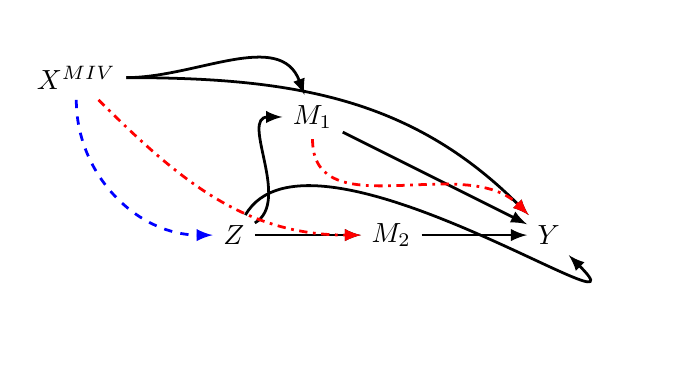
\begin{tikzpicture}[
    % Global config
    >=latex,
    line width=1pt,
    % Styles
    solid_black/.style={
        ->, 
        solid, 
        line width=1pt
    },
    dashed_blue/.style={
        ->, 
        dashed, 
        line width=1pt,
        blue
    },
    dash_dot_red/.style={
        ->, 
        dash dot, 
        line width=1pt,
        red
    }
]

% Nodes
\node (Z) at (0,0) {$Z$};
\node (X) at (-2,2) {$X^{MIV}$};
\node (M1) at (1,1.5) {$M_1$};
\node (M2) at (2,0) {$M_2$};
\node (Y) at (4,0) {$Y$};

% Paths
\draw[solid_black] (X) to[out=0,in=135] (Y);
\draw[solid_black] (X) to[out=0,in=110] (M1);
\draw[solid_black] (Z) to[out=30,in=180] (M1);
\draw[solid_black] (Z) to (M2);
\draw[solid_black] (M1) to (Y);
\draw[solid_black] (M2) to (Y);
\draw[solid_black] (Z) to[out=60,in=-45] (Y);

% Additional paths with styles
\draw[dashed_blue] (X) to[out=-90,in=180] (Z);
\draw[dash_dot_red] (X) to[out=-45,in=180] (M2);
\draw[dash_dot_red] (M1) to[out=-90,in=135] (Y);

\end{tikzpicture}

\end{document}